%%%%%%%%%%%%%%%%%%%%%%%%%%%%%%%%%%%%%%%%%
% Medium Length Professional CV
% LaTeX Template
% Version 2.0 (8/5/13)
%
% This template has been downloaded from:
% http://www.LaTeXTemplates.com
%
% Original author:
% Trey Hunner (http://www.treyhunner.com/)
%
% Important note:
% This template requires the resume.cls file to be in the same directory as the
% .tex file. The resume.cls file provides the resume style used for structuring the
% document.
%
%%%%%%%%%%%%%%%%%%%%%%%%%%%%%%%%%%%%%%%%%

%----------------------------------------------------------------------------------------
%	PACKAGES AND OTHER DOCUMENT CONFIGURATIONS
%----------------------------------------------------------------------------------------


\documentclass{resume2} % Use the custom resume2.cls style

\usepackage[left=0.75in,top=0.6in,right=0.75in,bottom=0.6in]{geometry} % Document margins
\usepackage{hyperref}
\usepackage{graphicx}
\usepackage{enumitem}


\name{Mario G\'omez Ramos} % Your name
\address{(+34)~628858474 \\ mgomez40@us.es}
\address{Nacido en: 08/02/1990}
\address{DNI: 28839143H}
\address{C/ Cristo de la Sed, 13  \\ Sevilla, Espa\~na CP 41005} % Your address
\photo{photo.png}
 % Your phone number and email



\begin{document}

%\begin{figure*}
%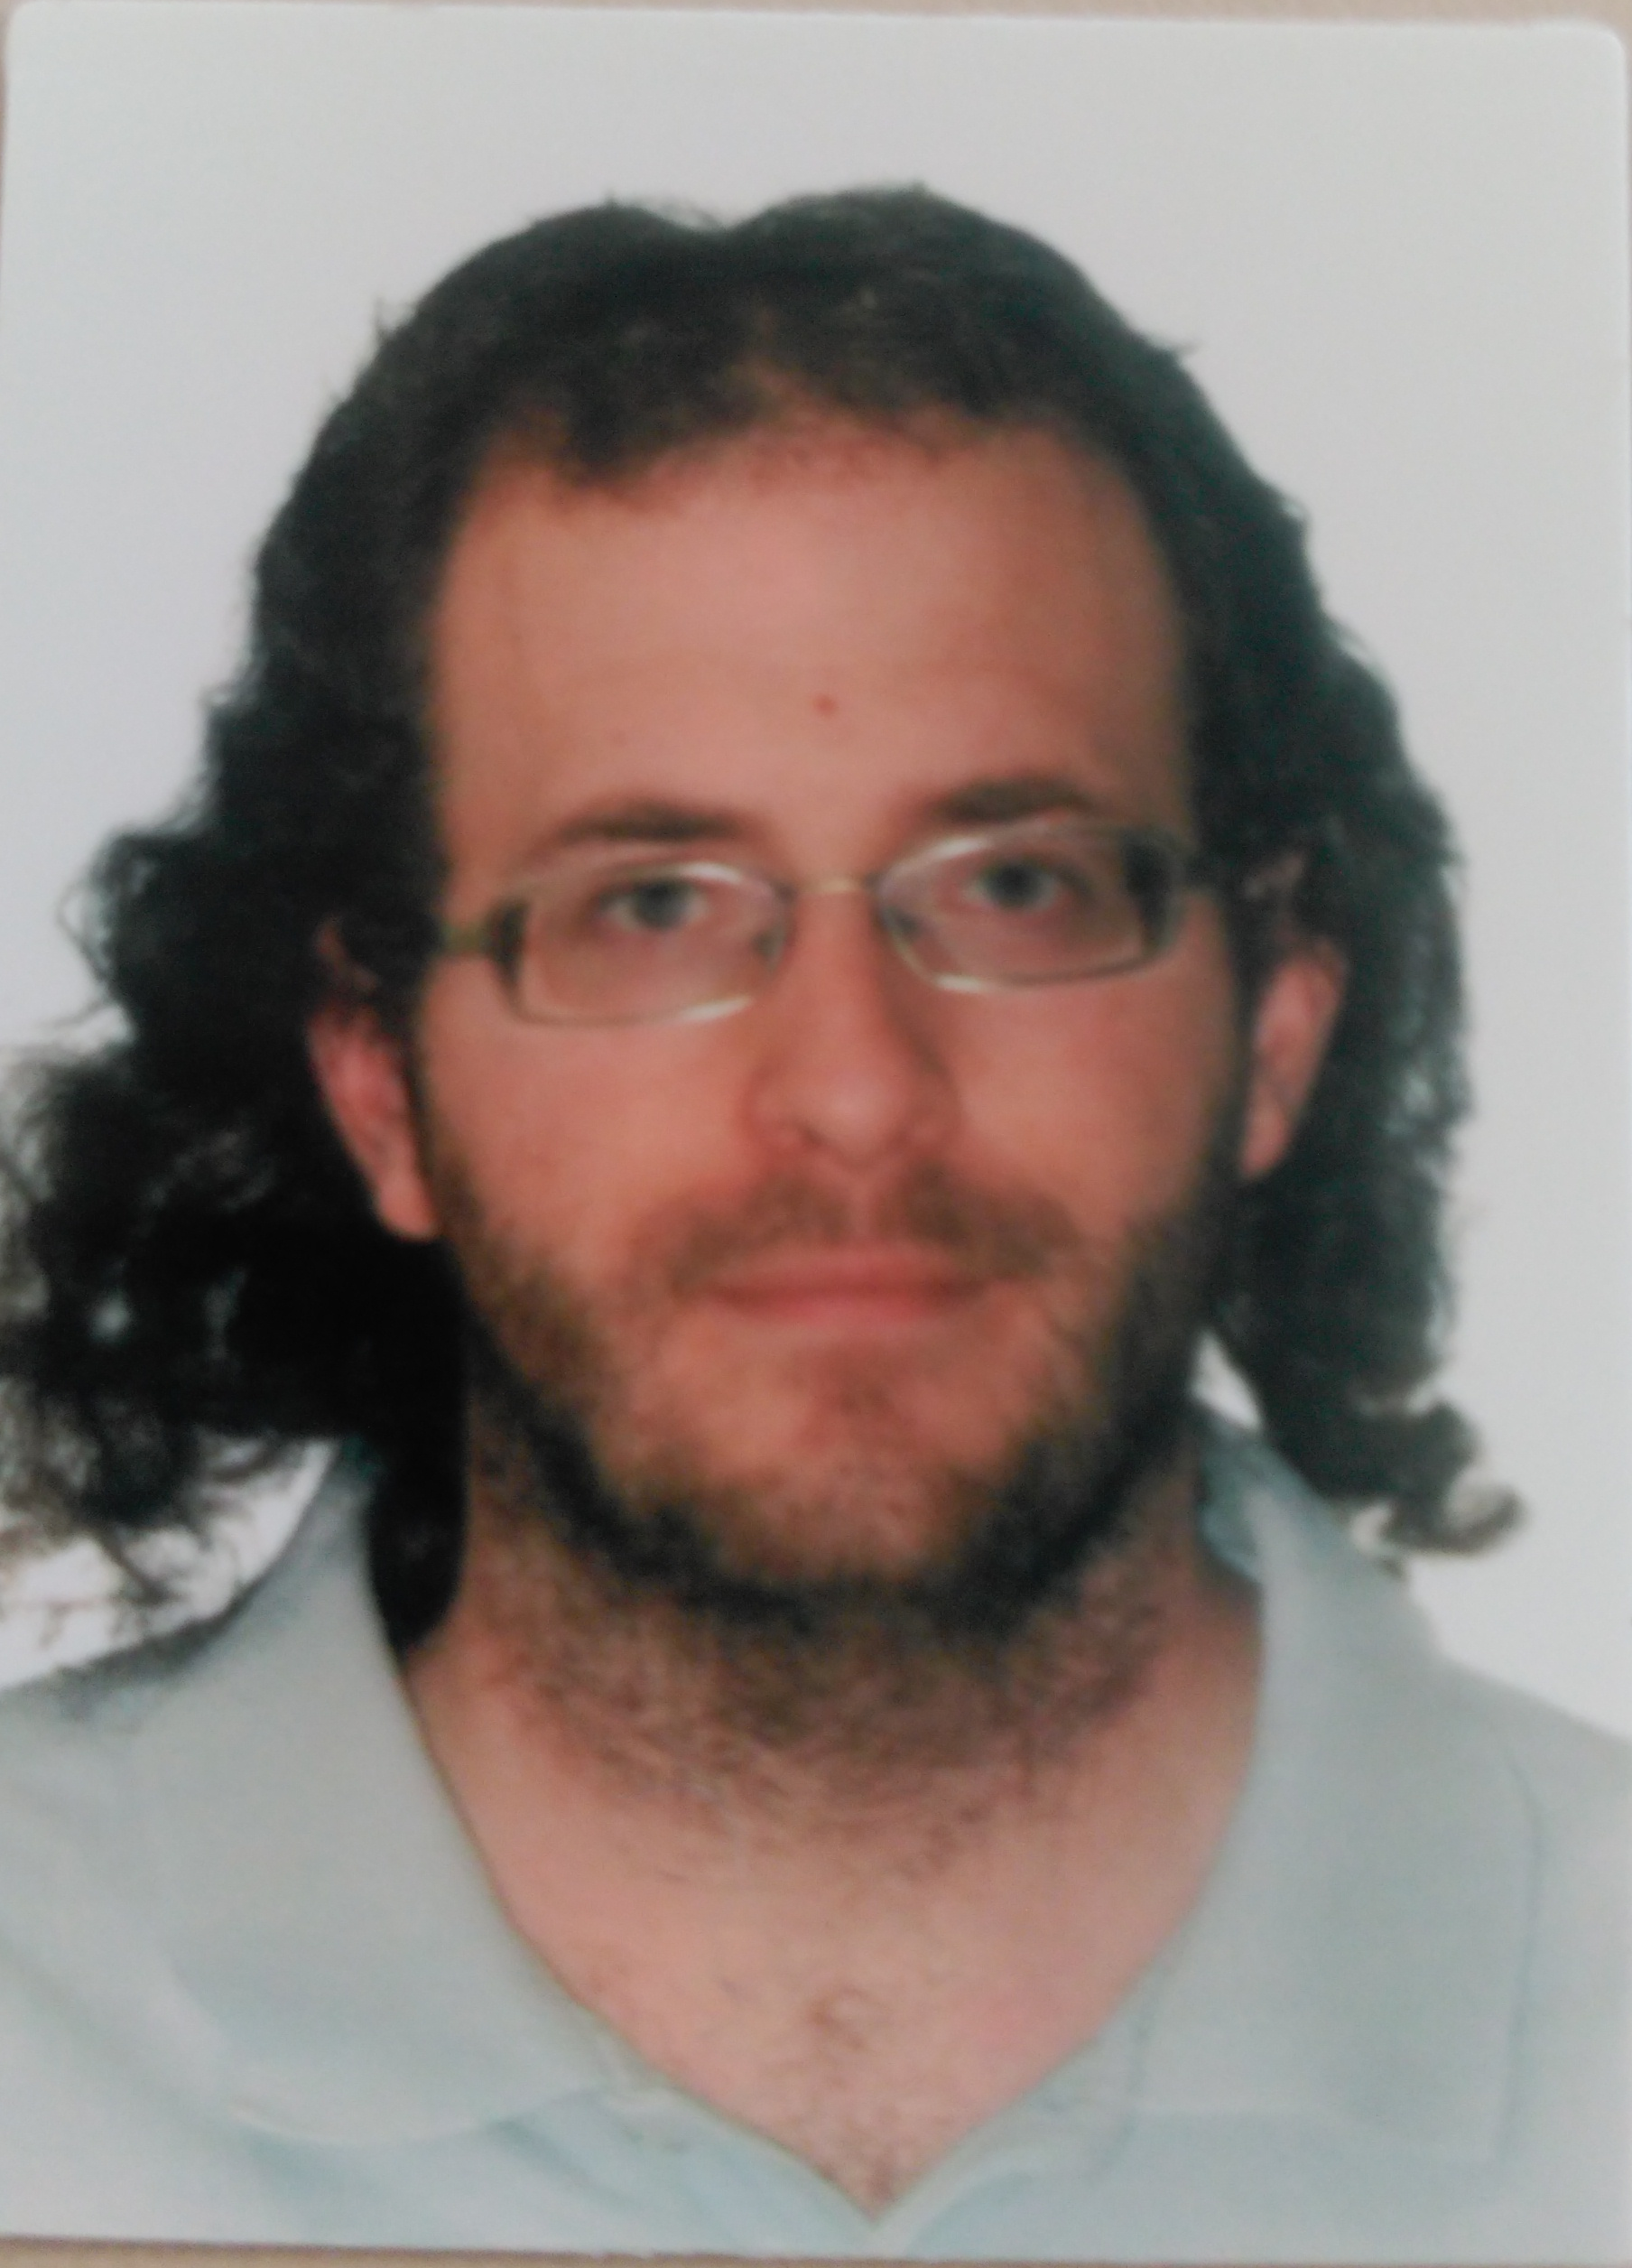
\includegraphics[width=0.1\textwidth]{photo.png}
%\end{figure*}

\begin{rSection}{Situaci\'on Profesional Actual}

{\sc Organismo:} Universidad de Sevilla\\
{\sc Departamento:} Departamento de F\'isica At\'omica, Molecular y Nuclear\\
{\sc Categor\'ia y fechas:} Profesor Permanente Laboral Interino desde el 01/05/2025\\
{\sc Direcci\'on postal:} Avda. Reina Mercedes s/n, Sevilla, Spain CP:1065\\
{\sc ORCID:} 0000-0002-9635-7818\hfill {\sc ResearcherID:} M-9164-2018\\
{\sc ScopusID:} 56720266500
\end{rSection}

%----------------------------------------------------------------------------------------
%	EDUCATION SECTION
%----------------------------------------------------------------------------------------

\begin{rSection}{1.~Historial Acad\'emico}
\begin{enumerate}[label=\alph*.]
\item Expediente Acad\'emico


{\bf Universidad de Sevilla} \hfill {\em 2008-2013} \newline
Licenciatura en F\'isica \newline
Nota media de expediente acad\'emico: 9.68/10\\
\\
{\bf Universidad de Sevilla, Universidad de Salamanca, Universidad Aut\'onoma de Madrid, Universidad de Barcelona, Universidad Complutense de Madrid, Universidad de Granada} \hfill {\em 2013-2014} \\ 
M\'aster Interuniversitario en F\'isica Nuclear \\
Nota media de expediente acad\'emico: 9.6/10\\
\\
{\bf Universidad de Sevilla} \hfill {\em 2014-2018} \\ 
Doctorado en Ciencias y Tecnolog\'ias F\'isicas \\
Calificaci\'on: Cum Laude 10/10\\

\item Titulaciones Universitarias


{\bf Universidad de Sevilla} \hfill {\em 08/2013} \newline
Licenciatura en F\'isica \newline
\\
{\bf Universidad de Sevilla, Universidad de Salamanca, Universidad Aut\'onoma de Madrid, Universidad de Barcelona, Universidad Complutense de Madrid, Universidad de Granada} \hfill {\em 08/2014} \\ 
M\'aster Interuniversitario en F\'isica Nuclear \\
\\
{\bf Universidad de Sevilla} \hfill {\em 11/2018} \\ 
Doctorado en Ciencias y Tecnolog\'ias F\'isicas \\

\item Becas y Contratos predoctorales

{\em 22/10/2014-21/10/2018} Becas de Formaci\'on de Personal Universitario (FPU) financiado por el Ministerio de Educaci\'on, Cultura y Deporte

\item Tesis doctoral

{\bf Universidad de Sevilla}\hfill{29/10/2018}\\
{\em A Transfer to the Continuum formalism for the study of $(p, pn)$ and $(p, 2p)$ reactions on unstable nuclei} \\
Calificaci\'on: Cum Laude 10/10\\


\item Menci\'on de doctorado europeo o internacional y/o menci\'on de calidad o excelencia del programa de doctorado.

Mención de \textbf{Doctorado Internacional}, Universidad de Sevilla

\item Premio extraordinario de doctorado

\item Otros t\'itulos y premios

\textbf{Premio extraordinario Fin de Carrera} de la Universidad de Sevilla por la Licenciatura en F\'isica\\

\textbf{Primer Premio Nacional de Fin de Carrera de Educaci\'on Universitaria} \\

\textbf{Premio extraordinario Fin de Estudios} de la Universidad de Sevilla por el M\'aster Universitario en F\'isica Nuclear 

\item Otros méritos de formación acad\'emica predoctoral o postdoctoral

{\sc \bf Cursos predoctorales:}
\begin{itemize}
\item FISMAT 2015 F\'isica y Matem\'aticas: Dos caras de una misma moneda (32 horas)
%\item Symmetries in Quantum Mechanics: Group Theory for Physicists (14 horas)
\item Introduction to High-Performance Computing (HPC) with OpenMP and MPI
(20 horas)
\item Lengua inglesa para la acreditación ISE III (140 horas)
\item Few-body Methods and Nuclear Reactions
\item 2016 GGI Lectures on Frontiers in Nuclear and Hadronic Physics (40 horas)

\end{itemize}

{\sc \bf Cursos postdoctorales:}

\end{enumerate}

\end{rSection}

%----------------------------------------------------------------------------------------
%	WORK EXPERIENCE SECTION
%----------------------------------------------------------------------------------------

\begin{rSection}{Historial y experiencia docente}

\begin{enumerate}[label=\alph*.]
\item Docecia impartida en grados y postgrados, licenciatura, doctorado

Hasta la fecha, el candidato tiene reconocida la impartici\'on de un total de 508.1 horas en grados y m\'asters de la Universidad de Sevilla (40.6 horas en Trabajos Fin de Grado y Fin de M\'aster)

{\bf Docencia impartida en el periodo predoctoral}

\begin{itemize}
\item F\'isica I en el Grado de \'Optica y Optometr\'ia y dobles grados asociados (60 horas)

\begin{itemize}
\item 2015-2016: 30 horas
\item 2016-2017: 30 horas
\end{itemize}

\item F\'isica Cu\'antica en el Grado en F\'isica y dobles grados asociados (60 horas)

\begin{itemize}
\item 2015-2016: 30 horas
\item 2016-2017: 30 horas
\end{itemize}

\end{itemize}

{\bf Docencia impartida en el periodo postdoctoral}

\begin{itemize}
\item F\'isica Cu\'antica en el Grado en F\'isica y dobles grados asociados (28 horas)

\begin{itemize}
\item 2020-2021: 10 horas
\item 2021-2022: 18 horas
\end{itemize}

\item F\'isica Nuclear y de Part\'iculas en el Grado en F\'isica y dobles grados asociados (161.5 horas)

\begin{itemize}
\item 2020-2021: 25 horas
\item 2021-2022: 16 horas
\item 2022-2023: 36.5 horas
\item 2023-2024: 44 horas
\item 2024-2025: 40 horas
\end{itemize}

\item F\'isica I en el Grado de Ingenier\'ia de Materiales (102 horas)

\begin{itemize}
\item 2021-2022: 30 horas
\item 2022-2023: 24 horas
\item 2023-2024: 24 horas
\item 2024-2025: 24 horas
\end{itemize}


\item Reacciones Nucleares en el M\'aster Universitario Erasmus Mundus en F\'isica Nuclear (25 horas)

\begin{itemize}
\item 2020-2021: 6 horas
\item 2021-2022: 6 horas
\item 2022-2023: 6 horas
\item 2023-2024: 7 horas
\end{itemize}

\item Introducci\'on a las Reacciones Nucleares en el M\'aster Universitario en F\'isica Nuclear (antiguo Erasmus Mundus) (7 horas)

\begin{itemize}
\item 2024-2025: 7 horas
\end{itemize}

\item Introducci\'on a las Reacciones Nucleares en el M\'aster Universitario en F\'isica Nuclear (24 horas)

\begin{itemize}
\item 2021-2022: 6 horas
\item 2022-2023: 6 horas
\item 2023-2024: 6 horas
\item 2024-2025: 6 horas
\end{itemize}

\end{itemize}

\item Direcci\'on de Trabajos de Fin de Grado, Fin de M\'aster, Diplomas de Estudios Avanzados, Tesinas de Licenciatura, etc.

{\bf Trabajos Fin de Grado}

\begin{itemize}
\item Evaluaci\'on de tasas de reacci\'on en procesos de captura radiativa de inter\'es astrof\'isico \\ 
{\sc Alumno:} Mario Osuna Mart\'inez\\
{\sc Tutores:} Mario G\'omez Ramos y Antonio Mat\'ias Moro Mu\~noz\\
{\sc Curso:} 2021-2022\\
{\sc Titulaci\'on:} Grado en F\'isica, Universidad de Sevilla

\item Descripci\'on cl\'asica de procesos subat\'omicos de dispersi\'on \\ 
{\sc Alumno:} Javier Carlos Ruiz Ramos\\
{\sc Tutores:} Mario G\'omez Ramos\\
{\sc Curso:} 2022-2023\\
{\sc Titulaci\'on:} Grado en F\'isica, Universidad de Sevilla

\item  Estudio de la reacci\'on de captura radiativa de inter\'es
astrof\'isico $^7$Be$(p, \gamma)^8$B mediante un modelo de dos cuerpos\\ 
{\sc Alumno:} Fernando D\'iaz Segado\\
{\sc Tutores:} Mario G\'omez Ramos y Antonio Mat\'ias Moro Mu\~noz\\
{\sc Curso:} 2022-2023\\
{\sc Titulaci\'on:} Grado en F\'isica, Universidad de Sevilla

\item  Nucleos\'intesis
de elementos pesados: el proceso s y el
proceso r\\ 
{\sc Alumno:} Ignacio Vioque Lombardo\\
{\sc Tutores:} Mario G\'omez Ramos \\
{\sc Curso:} 2023-2025\\
{\sc Titulaci\'on:} Grado en F\'isica, Universidad de Sevilla

\item  Estudio de $^9$Be con un modelo de
dos cuerpos en una base de
pseudoestados\\ 
{\sc Alumno:} Jes\'us \'Angel Luna C\'aceres\\
{\sc Tutores:} Mario G\'omez Ramos y Manuela Rodr\'iguez Gallardo\\
{\sc Curso:} 2024-2025\\
{\sc Titulaci\'on:} Grado en F\'isica, Universidad de Sevilla

\item  Din\'amica de la dispersi\'on
deuter\'on-n\'ucleo\\ 
{\sc Alumno:} Laura Bur\'on Malag\'on\\
{\sc Tutores:} Mario G\'omez Ramos y Antonio Mat\'ias Moro Mu\~noz\\
{\sc Curso:} 2024-2025\\
{\sc Titulaci\'on:} Doble Grado en F\'isica e Ingenier\'ia de Materiales, Universidad de Sevilla

\end{itemize}

{\bf Trabajos Fin de M\'aster}

\begin{itemize}
\item  Estudio del sistema prot\'on-neutr\'on y del
Berilio 11 en una base gaussiana compleja\\ 
{\sc Alumno:} Daniel Arjona Ni\~no\\
{\sc Tutores:} Jes\'us Casal Berbel, Mario G\'omez Ramos y Antonio Mat\'ias Moro Mu\~noz\\
{\sc Curso:} 2023-2024\\
{\sc Titulaci\'on:} M\'aster Universitario en F\'isica Nuclear por la UAM,UCM,UB,UGR,USAL y la
US

\end{itemize}

\item Evaluaciones positivas de la actividad docente.

El candidato ha sometido su docencia a evaluación en todos los cursos que ha impartido en la Universidad de Sevilla. De forma regular, se obtienen valoraciones por encima
del 8/10.

\item Material docente original y publicaciones docentes.

\item Elaboraci\'on/impartici\'on de cursos online en plataformas oficiales.

\item Proyectos de innovaci\'on docente.

\item Participaci\'on como ponente en congresos orientados a la formaci\'on docente universitaria.

\item Estancias como docente en diferentes centros.

\item Otros m\'eritos relacionados con la actividad y calidad docentes.

\end{enumerate}
\end{rSection}



%\begin{rSection}{Experience}

%\begin{rSubsection}{University of Seville}{February 2021 - }{Postdoctoral researcher}{Sevilla, Spain}
%\item Departamento de F\'isica At\'omica, Molecular y Nuclear, University of Seville
%\end{rSubsection}

%\begin{rSubsection}{Institut f\"ur Kernphysik}{May 2019 - January 2021}{Humboldt Fellow}{Darmstadt, Germany}
%\item Financed by the Alexander von Humboldt Foundation
%\end{rSubsection}

%\begin{rSubsection}{University of Seville}{January 2019 - March 2019}{Postdoctoral researcher}{Sevilla, Spain}
%\item Departamento de F\'isica At\'omica, Molecular y Nuclear, University of Seville
%\end{rSubsection}

%\begin{rSubsection}{University of Seville}{October 2014 - October 2018}{Predoctoral student/researcher}{Sevilla, Spain}
%\item Financed by the FPU Grant from the Spanish Ministry of Education, Culture and Sport
%\end{rSubsection}

%\end{rSection}

\begin{rSection}{Historial y experiencia investigadora}
\begin{enumerate}[label=\alph*.]
\item Libros.

\item Cap\'itulos de libros (excluyendo actas de congresos)

\item Art\'iculos publicados en revistas cient\'ificas internacionales (JCR)

{\sc Resumen}

\begin{itemize}
\item Ar\'iculos en revistas indexadas: 32

\item Proceedings: 7

\item Citas (WoS): 404

\item \'Indice h (WoS): 13
\end{itemize}

{\sc Publicaciones}

\begin{enumerate}[label=\arabic*.]
\item A.M. Moro, J. Casal and {\bf M. G\'omez-Ramos}, {\it The art of modeling nuclear reactions with weakly bound nuclei: status and perspectives}, The European Physics Journal A {\bf 61}, 47 (2025) DOI: \url{https://doi.org/10.1140/epja/s10050-025-01500-0}

\item J. Casal, {\bf M. G\'omez-Ramos} and  A.M. Moro, {\it Collective core effects and dineutron correlations in three-body nuclei}, Nuovo Cimento C {\bf 47}, 41 (2024) DOI:\url{https://doi.org/10.1393/ncc/i2024-24041-0}

\item {\bf M. G\'omez-Ramos}, {\it Eikonal calculation of (p, 3p) cross sections for neutron-rich nuclei}, Physical Review C {\bf 109}, 064622 (2024) DOI: \url{https://doi.org/10.1103/PhysRevC.109.064622}

\item B.D. Linh, A. Corsi,... {\bf M. G\'omez-Ramos} \textit{et al.}, {\it Onset of collectivity for argon isotopes close to N = 32}, Physical Review C {\bf 109}, 034312 (2024) DOI: \url{https://doi.org/10.1103/PhysRevC.109.034312}



\item N. Timofeyuk and {\bf M. G\'omez-Ramos}, {\it Cluster scattering in the non-local model}, Frontiers in Physics {\bf 11}, 1197726 DOI: \url{https://doi.org/10.3389/fphy.2023.1197726}

\item {\bf M. G\'omez-Ramos}, J. G\'omez-Camacho, A.M. Moro , {\it Isospin dependence in single-nucleon removal cross sections explained through valence-core destruction effects}, Physics Letters B {\bf 847}, 138284 (2023) DOI: \url{https://doi.org/10.1016/j.physletb.2023.138284}

\item A.~Corsi, Y.~Kubota,...{\bf M. G\'omez-Ramos} {\it et al}, {\it Searching for universality of dineutron correlation at the surface of Borromean nuclei}, Physics Letters B {\bf 840}, 137875 (2023) DOI: \url{https://doi.org/10.1016/j.physletb.2023.137875}

\item T.~Pohl, Y.L.~Sun,...{\bf M. G\'omez-Ramos} {\it et al}, {\it Multiple Mechanisms in Proton-Induced Nucleon Removal at $\sim$100 MeV/Nucleon}, Physical Review Letters {\bf 130}, 172501 (2023) DOI: \url{https://doi.org/10.1103/PhysRevLett.130.172501}

\item N.~K. Timofeyuk, L.~Moschini, {\bf M. G\'omez-Ramos}, {\it Single-particle spectroscopic strength from nucleon transfer reactions with a three-nucleon force contribution}, Physics Letters B {\bf 839}, 137815 (2023) \url{https://doi.org/10.1016/j.physletb.2023.137815}

\item {\bf M. G\'omez-Ramos}, J. G\'omez-Camacho, A.M. Moro , {\it Binding-energy asymmetry in absorption explored through CDCC extended for complex potentials}, Physics Letters B {\bf 832}, 137252 (2022) DOI: \url{https://doi.org/10.1016/j.physletb.2022.137252}

\item Vinicius Antonio Bocaline Zagatto, {\bf M. G\'omez-Ramos} \textit{et al.} {\it Elastic, inelastic, and one-neutron transfer angular distributions of $^6\mathrm{Li}+^{120}\mathrm{Sn}$ at energies near the Coulomb barrier}, Physical Review C \textbf{106}, 014622 (2022) DOI: \url{https://doi.org/10.1103/PhysRevC.106.014622}

\item T. Aumann, W. Bartmann,... {\bf M. G\'omez-Ramos} \textit{et al.} {\it PUMA, antiProton unstable matter annihilation} 
The European Physics Journal A \textbf{58}, 88 (2022) DOI: \url{https://doi.org/10.1140/epja/s10050-022-00713-x}

\item B.D. Linh, A. Corsi,... {\bf M. G\'omez-Ramos} \textit{et al.} {\it Investigation of the ground-state spin inversion in the $^{47-49}$Cl neutron-rich  isotopes}, Physical Review C \textbf{104}, 044331 (2021) DOI: \url{https://doi.org/10.1103/PhysRevC.104.044331}

\item J. Casal, {\bf M. G\'omez-Ramos} {\it Opening angle and dineutron correlations in knockout reactions with Borromean two-neutron halo nuclei}, Physical Review C \textbf{104}, 024618 (2021) DOI: \url{https://doi.org/10.1103/PhysRevC.104.024618}

\item T. Aumann, C. Barbieri, D. Bazin, C.A. Bertulani, A. Bonaccorso, W.H. Dickhoff, A. Gade, {\bf M. Gómez-Ramos}, B.P. Kay, A.M. Moro, T. Nakamura, A. Obertelli, K. Ogata, S. Paschalis, T. Uesaka
{\it Quenching of single-particle strength from direct reactions with stable and rare-isotope beams}, Prog. Part. Nucl. Phys. \textbf{118}, 103847 (2021) DOI: \url{https://doi.org/10.1016/j.ppnp.2021.103847}

\item {\bf M. G\'omez-Ramos},  A. Obertelli and Y.L. Sun
 {\it Breakup reactions and their ambiguities}, The European Physics Journal A \textbf{57}, 148 (2021) DOI: \url{https://doi.org/10.1140/epja/s10050-021-00446-3}

\item {\bf M. G\'omez-Ramos}, J. G\'omez-Camacho, J. Lei and A.M. Moro
 {\it The Hussein–McVoy formula for inclusive breakup revisited}, The European Physics Journal A \textbf{57}, 57 (2021) DOI: \url{https://doi.org/10.1140/epja/s10050-021-00376-0}

\item {\bf M. G\'omez-Ramos}, A. Deltuva and A.M. Moro {\it Benchmarking Faddeev and transfer-to-the-continuum calculations for $(p,pN)$ reactions}, Physical Review C \textbf{102}, 064613 (2020) DOI: \url{https://doi.org/10.1103/PhysRevC.102.064613}


\item Axel Frotscher, {\bf M. G\'omez-Ramos}, Alexandre Obertelli  \textit{et al}, {\it Sequential nature of (p,3p) two-proton knockout from neutron-rich nuclei}, Physical Review Letters {\bf 125}, 012501 (2020) DOI: \url{https://doi.org/10.1103/PhysRevLett.125.012501}

%\url{https://link.aps.org/doi/10.1103/PhysRevLett.125.012501}



\item {\bf M. G\'omez-Ramos} and N.~K. Timofeyuk, {\it Perey-effect in continuum-discretized coupled-channel description of (d, p)
reactions}, Journal of Physics G: Nuclear and Particle Physics {\bf 46}, 085102 (2019)  DOI: \url{https://doi.org/10.1088/1361-6471/ab25c5}

%\url{https://doi.org/10.1088\%2F1361-6471\%2Fab25c5}\hfill {\sc CIT} (ISI):1

\item A.M. Moro, J. Casal and {\bf M. G\'omez-Ramos}, {\it Investigating the $^{10}$Li continuum through
$^9$Li$(d,p)^{10}$Li reactions}, Physics Letters B {\bf 793}, 13 (2019)  DOI: \url{https://doi.org/10.1016/j.physletb.2019.04.015}

%\url{https://doi.org/10.1016/j.physletb.2019.04.015}\hfill {\sc CIT} (ISI):5

\item A. Corsi, Y. Kubota, J. Casal, {\bf M. G\'omez-Ramos}, A.M. Moro \textit{et al}, {\it Structure of $^{13}$Be probed
via quasi-free scattering}, Physics Letters B {\bf 797}, 134843 (2019) DOI: \url{https://doi.org/10.1016/j.physletb.2019.134843}


\item J. G\'omez-Camacho, {\bf M. G\'omez-Ramos}, J. Casal and A.M. Moro {\it Time scales in nuclear structure and nuclear reactions of exotic nuclei}, Nuovo Cimento C {\bf 42}, 86 (2019) DOI: \url{https://doi.org/10.1393/ncc/i2019-19086-9}
%\url{https://doi.org/10.1016/j.physletb.2019.134843}\hfill {\sc CIT} (ISI):1

\item {\bf M. G\'omez-Ramos} and A.M. Moro, {\it Binding-energy independence of reduced spectroscopic strengths derived from $(p, 2p)$ and $(p, pn)$ reactions with nitrogen and oxygen isotopes}, Physics Letters B {\bf 785}, 511 (2018) DOI: \url{https://doi.org/10.1016/j.physletb.2018.08.058}

%\url{https://doi.org/10.1016/j.physletb.2018.08.058}\hfill {\sc CIT} (ISI):7

\item {\bf M. G\'omez-Ramos} and N. Timofeyuk {\it Reduced sensitivity of the $(d,p)$ cross sections to the deuteron model beyond the adiabatic approximation}, Phys. Rev. C {\bf 98}, 011601(R) (2018) DOI: \url{https://doi.org/10.1103/PhysRevC.98.011601}

%\url{https://doi.org/10.1103/PhysRevC.98.011601}\hfill {\sc CIT} (ISI):6

\item K. Yoshida, {\bf M. G\'omez-Ramos}, {K. Ogata} and A.M. Moro, {\it Benchmarking theoretical formalisms
for $(p,pn)$ reactions: The $^{15}$C$(p,pn) ^{14}$C case.}, Phys. Rev. C {\bf 97}, 024608 (2018) DOI: \url{https://doi.org/10.1103/PhysRevC.97.024608}

%\url{https://doi.org/10.1103/PhysRevC.97.024608}\hfill {\sc CIT} (ISI):5

\item {\bf M. G\'omez-Ramos}, J. Casal and A.M. Moro, {\it Linking structure and dynamics in $(p,pn)$ reactions
with Borromean nuclei: The $^{11}$Li$(p,pn)^{10}$Li case.}, Physics Letters B {\bf 772}, 115 (2017) DOI: \url{https://doi.org/10.1016/j.physletb.2017.06.023}

%\url{https://doi.org/10.1016/j.physletb.2017.06.023}\hfill {\sc CIT} (ISI):7

\item J. Casal, {\bf M. G\'omez-Ramos} and A.M. Moro, {\it Description of the $^{11}$Li$(p,d)^{10}$Li transfer reaction using structure overlaps from a full three-body model.}, Physics Letters B {\bf 767}, 307 (2017) DOI: \url{https://doi.org/10.1016/j.physletb.2017.02.017}

%\url{https://doi.org/10.1016/j.physletb.2017.02.017}\hfill {\sc CIT} (ISI):12

\item {\bf M. G\'omez-Ramos} and A.M. Moro {\it Influence of target deformation and deuteron breakup in $(d, p)$ transfer reactions.}, Phys. Rev. C {\bf 95}, 044612 (2017) DOI: \url{https://doi.org/10.1103/PhysRevC.95.044612}

%\url{https://doi.org/10.1103/PhysRevC.95.044612}\hfill {\sc CIT} (ISI):6

\item {\bf M. G\'omez-Ramos} and {A.M. Moro}, {\it Interplay of projectile breakup and target excitation in reactions induced by weakly bound nuclei.}, Phys. Rev. C {\bf 95}, 034609 (2017) DOI: \url{https://doi.org/10.1103/PhysRevC.95.034609}

%\url{https://doi.org/10.1103/PhysRevC.95.034609}\hfill {\sc CIT} (ISI):9

\item A.M. Moro, J. Lei, {\bf M. G\'omez-Ramos}, J.M. Arias, R. de Diego, J. G\'omez-Camacho and J.A. Lay,
{\it Recent Developments for the Calculation of Elastic and Non-elastic Breakup of Weakly-Bound Nuclei.},
Acta Physica Polonica B {\bf 47}, 821 (2016) DOI: \url{https://doi.org/10.5506/APhysPolB.47.821}

%\url{https://doi.org/10.5506/APhysPolB.47.821}



\item {\bf M. G\'omez-Ramos}, A.M. Moro, J. G\'omez-Camacho and I.J. Thompson, {\it Transfer induced by core
excitation within an extended DWBA method.}, Phys. Rev. C {\bf 92}, 014613 (2015) DOI: \url{https://doi.org/10.1103/PhysRevC.92.014613}

%\url{https://doi.org/10.1103/PhysRevC.92.014613}\hfill {\sc CIT} (ISI):13
\end{enumerate}

{\sc Proceedings:}

\begin{enumerate}[label=\arabic*.]

\item K.C.Z. Haverson, R. Smith,... {\bf M. G\'omez-Ramos} \textit{et al.},  {\it Searching for particle-hole cluster bands in 8Be using the ISOLDE Solenoidal Spectrometer}, EPJ Web of Conferences {\bf 311} 00012 (2024) DOI: \url{https://doi.org/10.1051/epjconf/202431100012}

\item {\bf M. G\'omez-Ramos}, J. G\'omez-Camacho and  A.M. Moro,  {\it Core-valence absorption in breakup and stripping reactions and its isospin dependence}, EPJ Web of Conferences 290, 02019 (2023) DOI: \url{https://doi.org/10.1051/epjconf/202329002019}

\item J. Casal, {\bf M. G\'omez-Ramos} and  A.M. Moro,  {\it Dineutron correlations in knockout reactions with Borromean halo nuclei}, EPJ Web of Conferences 290, 09006 (2023) DOI: \url{https://doi.org/10.1051/epjconf/202329009006}

\item J. Casal, {\bf M. G\'omez-Ramos},  A.M. Moro and A. Corsi, {\it Exploring continuum structures in reactions with three-body nuclei},  Journal of Physics Conference Series {\bf 1643}, 012075 (2020) DOI: \url{https://doi.org/10.1088/1742-6596/1643/1/012075}

\item A.M. Moro, J. Lei and {\bf M. G\'omez-Ramos}, {\it Reaction theory and advanced CDCC},  Journal of Physics Conference Series {\bf 1643}, 012100 (2020) DOI: \url{https://doi.org/10.1088/1742-6596/1643/1/012100}

\item {\bf M. G\'omez-Ramos} and A.M. Moro, {\it Transfer to the Continuum Calculations of Quasifree (p, pn) and (p, 2p) Reactions at Intermediate and High Energies}, Libro: R\'ABIDA 2015: Basic Concepts in Nuclear Physics: Theory, Experiments and Applications,  Springer Proceedings in Physics {\bf 182}, 171 (2016) DOI: \url{https://doi.org/10.1007/978-3-319-21191-6_6} 

\item {\bf M. G\'omez-Ramos} and A.M. Moro, {\it Transfer to the continuum calculations of quasifree (p,pn) and (p,2p) reactions}, Libro: 12th International Conference on Nucleus-Nucleus Collisions 2015, EPJ Web of Conferences {\bf 117} (2016), DOI: \url{https://doi.org/10.1051/epjconf/201611706024}

\end{enumerate}

\item Participaci\'on en proyectos de investigaci\'on financiados.

\begin{enumerate}[label=\arabic*.]

\item {\sc T\'itulo}: Reacciones Inducidas por interacciones Electrodébiles y Nucleares a energías bajas
e intermedias (RibEN) {\bf (PID2023-146401NB-I00)}\\
{\sc Financiado por}: Ministerio de Ciencia, Educaci\'on y Universidades.\\
{\sc Desde}: 01/09/2024\hfill {\sc Hasta}: 31/12/2027\\
{\sc Rol}: Equipo de Investigación\\
{\sc IP}: Guillermo D. Meg\'ias V\'azquez, Jos\'e Antonio Lay Valera\\
\item {\sc T\'itulo}: EUROpean Laboratories for Accelerator Based Science - EURO-LABS
{\bf( 4598/1176)}\\
{\sc Financiado por}: European Commission.\\
{\sc Desde}: 01/09/2022\hfill {\sc Hasta}: 31/08/2026\\
{\sc Rol}: Investigador Postdoctoral\\
{\sc IP}: Manuela Rodr\'iguez Gallardo\\
\item {\sc T\'itulo}: Procesos de dispersión fuerte, electromagnética y débil con núcleos a energías bajas e intermedias
{\bf(PID2020-114687GB-I00)}\\
{\sc Financiado por}: Ministerio de Ciencia e Innovación.\\
{\sc Desde}: 01/09/2021\hfill {\sc Hasta}: 31/08/2024\\
{\sc Rol}: Equipo de Trabajo\\
{\sc IP}: Manuela Rodr\'iguez Gallardo and Juan Antonio Caballero Carretero\\
\item {\sc T\'itulo}: Reacciones y Estructura nucleares: interaccion Neutrino-nucleo, Abundancias elementales del Cosmos, evolucion Estelar y procesos Radiativos (RENACER)
{\bf(P20\_01247)}\\
{\sc Financiado por}: Junta de Andaluc\'ia.\\
{\sc Desde}: 05/10/2021\hfill {\sc Hasta}: 31/03/2023\\
{\sc Rol}: Equipo Colaborador\\
{\sc IP}: Manuela Rodr\'iguez Gallardo\\
\item {\sc T\'itulo}: European Nuclear Science and Application Research 2 (ENSAR2)
{\bf(H2020-INFRAIA-2014-2015)}\\
{\sc Subgrupo}: Theoretical Support for Nuclear Facilities in Europe (TheoS)\\
{\sc Financiado por}: European Comission.\\
{\sc Desde}: 01/03/2016\hfill {\sc Hasta}: 29/02/2020\\
{\sc Rol}: Contratado Postdoctoral\\
{\sc IP}: Muhsin Harakeh\\
{\sc IP subgrupo}: Antonio M. Moro\\
\item {\sc T\'itulo}: Estudios de Procesos de Dispersi\'on Fuerte y Electrod\'ebil con N\'ucleos
a Energ\'ias Bajas e Intermedias {\bf (FIS2017-88410-P)}\\
{\sc Financiado por}: Ministerio de Economía\\
{\sc Desde}: 01/01/2018\hfill {\sc Hasta}: 31/09/2021\\
{\sc Rol}: Equipo de Trabajo\\
{\sc IP}: Antonio M. Moro and J. A. Caballero\\
\item {\sc T\'itulo}: Estructura de N\'ucleos, Mol\'eculas y Hadrones y su Din\'amica en Procesos de
Dispersi\'on Fuerte y Electrod\'ebil {\bf (FIS2014-53448-C2-1-P)}\\
{\sc Financiado por}: Ministerio de Econom\'ia\\
{\sc Desde}: 01/01/2015\hfill {\sc Hasta}: 30/06/2018\\
{\sc Rol}: Equipo de Trabajo\\
{\sc IP}: Antonio M. Moro and J. A. Caballero\\
\item {\sc T\'itulo}:  La F\'isica Nuclear Fuera del Valle de Beta-Estabilidad: Sus Implicaciones en
Astrof\'isica {\bf (P11-FQM-7632)}\\
{\sc Financiado por}: Junta de Andaluc\'ia\\
{\sc Desde}: 26/03/2013\hfill {\sc Hasta}: 31/03/2018\\
{\sc Rol}: Investigador\\
{\sc IP}: Manuel Luis Lozano Leyva\\
\item {\sc T\'itulo}:  Desarrollos en Teor\'ia de Reacciones y C\'alculos para la Interpretaci\'on de
Experimentos con N\'ucleos Ex\'oticos {\bf (FIS2013-41994-P)}\\
{\sc Financiado por}: Ministerio de Economía\\
{\sc Desde}: 01/01/2014\hfill {\sc Hasta}: 31/12/2016\\
{\sc Rol}: Equipo de Trabajo\\
{\sc IP}: Antonio M. Moro \\
\\
%\item {\sc T\'itulo}: SFB 1245: From Fundamental Interactions to Structure and Stars\\
%{\sc Financiado por}: Deutsche Forschungsgemeinschaft\\
%{\sc Desde}: 2016\\
%{\sc Portavoz}: Achim Schwenk \\
%\\
%\\
\end{enumerate}

\item Becas y contratos postdoctorales.

\begin{rSubsection}{Universidad de Sevilla}{01/05/2022 - 30/04/2025}{Investigador Postdoctoral}{Sevilla, Espa\~na}
\item Contrato postdoctoral del programa Juan de la Cierva Incorporaci\'on del Ministerio de Ciencia e Innovaci\'on
\end{rSubsection}

\begin{rSubsection}{Universidad de Sevilla}{01/02/2021 - 30/04/2022}{Investigador Postdoctoral}{Sevilla, Espa\~na}
\item Contrato postdoctoral del programa PAIDI DOCTOR de la Junta de Andaluc\'ia
\end{rSubsection}

\begin{rSubsection}{Institut f\"ur Kernphysik}{01/05/2019 - 31/01/2021}{Humboldt Fellow}{Darmstadt, Alemania}
\item Financiado por el programa AvH Fellowships for Young Researchers de la Fundaci\'on Alexander von Humboldt
\end{rSubsection}

\begin{rSubsection}{Universidad de Sevilla}{15/12/2018 - 04/03/2019}{Postdoctoral researcher}{Sevilla, Espa\~na}
\item Contratado por el proyecto ENSAR2
\end{rSubsection}

\item Pertenencia a grupos de investigación.

\begin{itemize}
\item Pertenencia al Grupo F\'isica Nuclear B\'asica FQM-160 \\
IP: Jos\'e Miguel Arias Carrasco
\end{itemize}

\item Direcci\'on de tesis doctorales.

\item Estancias en centros de investigaci\'on.

\begin{itemize}
%\item  Universidad de Surrey, Reino Unido (Supervisor: N. Timofeyuk) \newline Investigador postdoctoral, Nov 2018 - Dic 2018 
%\newline\quad\quad {\it Extension of Perey factors to CDCC calculations}

\item Universidad de Surrey, Reino Unido (Supervisor: N. Timofeyuk) \newline Investigador predoctoral, Oct 2017 - Dic 2017 
\newline\quad\quad {\it Study of non-locality in CDCC calculations}

\item  Research Center for Nuclear Physics, Osaka , Jap\'on (Supervisor: K. Ogata) \newline Investigador predoctoral, Feb 2017 - Mar 2017 
\newline\quad\quad {\it Benchmark between TC and DWIA}
\end{itemize}

\item  Actividad de evaluación para revistas indexadas en el JCR.

Actividad como referee \textit{(Debido a que APS no presenta certificados de referee y que en las revistas de Elsevier y Springer los distintos artículos se revisaron con perfiles temporales creados por los editores no se presenta certificado para este apartado)}:

\begin{itemize}
\item Physical Review C (42 art\'iculos revisados)

\item The European Physics Journal A (7 art\'iculos revisados)

\item Journal of Physics G (2 art\'iculos revisados)

\item Nuclear Physics A (1 art\'iculo revisado)

\item Turkish Journal of Physics (1 art\'iculo revisado)

\item Europhysics Letters (1 art\'iculo revisado)

\item Progress in Theoretical and Experimental Physics (1 art\'iculo revisado)

\item Physics Letters B (1 art\'iculo revisado)

\item Communications in Theoretical Physics (1 art\'iculo revisado)

\item International Journal of Modern Physics E (1 art\'iculo revisado)

\end{itemize}

\item Publicaciones en actas de congresos o reuniones científicas

\begin{itemize}
\item Ponencia invitada presentada por el concursante a la plaza.
\begin{enumerate}[label=\arabic*.]
\item {\it Core-valence absorption in breakup and stripping reactions and its
isospin dependence} 
\newline {\sc Conferencia}: EUropean Nuclear Physics Conference 2022 (EUNPC22), Santiago de Compostela, Espa\~na, Oct 2022
\end{enumerate}

\item Ponencia oral presentada por el concursante a la plaza.

\begin{enumerate}[label=\arabic*.]

\item {\it Core destruction effects in nucleon removal reactions} 
\newline {\sc conferencia}: XXXIX Reuni\'on Bienal de la Real Sociedad Española de F\'isica, San Sebasti\'an, Espa\~na, Jul 2024

\item {\it Effect of valence-core destruction in the dependence on isospin asymmetry for single-nucleon knockout “quenching” factor} 
\newline {\sc Conferencia}: Direct Reactions on Exotic Beams 2024 (DREB2024), Wiesbaden, Alemania, Jun 2024



\item {\it Core-valence absorption in breakup reactions: a source of
binding-energy asymmetry in nucleon removal observables?} 
\newline {\sc Conferencia}: Direct Reactions on Exotic Beams 2022 (DREB2022), Santiago de Compostela, Espa\~na, Jul 2022

\item {\it Analysis of isospin dependence of “quenching factors” for $(p, pn)$ and $(p, 2p)$ reactions via the Transfer to the Continuum formalism} 
\newline {\sc Conferencia}: Direct Reactions on Exotic Beams 2018 (DREB2018), Matsue, Jap\'on, Jun 2018

\item {\it Study of “quenching factors” for $(p, pn)$ and $(p, 2p)$ reactions
through the Transfer to the Continuum formalism} 
\newline {\sc Conferencia}: Recent advances and challenges in the description of nuclear reactions at the limit of stability, Trento, Italia, Mar 2018

\item {\it Transfer to the continuum calculations of $(p, pN )$ reactions on Borromean nuclei} 
\newline {\sc Conferencia}: 5$^{\rm th}$ UK Nuclear Theory Meeting, York, Reino Unido, Nov 2017

\item {\it Transfer to the continuum calculations of $(p, pn)$ and $(p, 2p)$ reactions at intermediate and high energies} 
\newline {\sc Conferencia}: 3$^{\rm rd}$ International Workshop on Quasifree Scattering
with Radioactive-Ion Beams (QFS-RB 17), York, Reino Unido, Jul 2017

\item {\it Transfer to the continuum calculations for $(p, pN)$ and transfer reactions on Borromean nuclei} 
\newline {\sc conferencia}: XXXVI Reuni\'on Bienal de la Real Sociedad Española de F\'isica, Santiago de Compostela, Espa\~na, Jul 2017

\item {\it Transfer to the continuum calculations for $(p, pN )$ and transfer reactions on Borromean nuclei} 
\newline {\sc conferencia}: VIII CPAN Days, Zaragoza, Espa\~na, Nov 2016

\item {\it Transfer to the continuum calculations of $(p, pN )$ reactions} 
\newline {\sc conferencia}: Direct Reactions on Exotic Beams 2016 (DREB2016), Halifax, Canad\'a, Jul 2016
 


\item{\it Transfer to the continuum calculations of quasifree $(p, pn)$ and $(p, 2p)$ reactions at intermediate and high energies} 
\newline {\sc conferencia}: International Scientific Meeting on Nuclear Physics
(RABIDA15), “Basic concepts in Nuclear Physics: theory, experiments
and applications”, La R\'abida (Huelva), Espa\~na, Jun 2015

\item{\it Scattering and structure of quantum systems within few-body models} 
\newline {\sc conferencia}: Complex Systems: from the Nanoscale to the Continuum (CS:N2C),M\"unster, Alemania, Feb 2015


 \end{enumerate}

\item  Comunicación con p\'oster.

\begin{enumerate}[label=\arabic*.]

\item {\it Interplay between breakup of weakly bound nuclei and collective excitations} 
\newline {\sc conferencia}: Direct Reactions on Exotic Beams 2016 (DREB2016), Halifax, Canad\'a, Jul 2016

\item {\it Transfer to the continuum calculations of quasifree $(p, pn)$ and $(p, 2p)$ reactions} 
\newline {\sc conferencia}: 12th International Conference on Nucleus-Nucleus collisions (NN2015), Catania, Italia, June 2015

\item{\it Dynamical effects for thransfer reactions in the DWBA approximation} 
\newline{\sc conferencia}: Euroschool on Exotic Beams 2014, Padova, Italia, Sep 2014

\end{enumerate}

\item Edici\'on de actas

\end{itemize}

\item Seminarios invitados impartidos en centros de prestigio.

\begin{enumerate}[label=\arabic*.]

%\item {\it $(p, pN )$ reactions: application to the “quenching” puzzle and to
%reactions on Borromean nuclei}, Universidad de Manchester, Reino Unido, Nov 2018

%\item {\it $(p, pN )$ reactions analyzed with the Transfer to the Continuum
%formalism. The “quenching” puzzle and application to Borromean
%nuclei}, Universidad de York, Reino Unido, Nov 2018


\item {\it Transfer to the continuum calculations of $(p,pN)$ reactions at intermediate and high energies}, Universidad de Sevilla, Espa\~na, Jun 2015

\end{enumerate}


\item Premios de investigación.

\item Investigador Principal de proyectos internacionales.

\item  Investigador principal de proyectos nacionales.

\item Investigador principal de proyectos autonómicos.

\item Responsable de grupos de investigación.

\item Organización de congresos científicos.

[Mar-Jun 2020] Co-organizador de los seminarios online ``Nuclear Reaction Seminars'' \url{https://reactionseminar.github.io/}

\end{enumerate}
\end{rSection}

\begin{rSection}{Historial y experiencia en transferencia e intercambio de conocimiento a la sociedad}

\begin{enumerate}[label=\alph*.]

\item  Patentes y productos con registro de propiedad intelectual.

\item Participación en proyectos nacionales o internacionales de transferencia.

\item Participación en contrato con empresas.

\item Actividades de divulgación científica.

\begin{itemize}
\item Participaci\'on habitual en las actividades de divulgaci\'on de la facultad de F\'isica:
\begin{itemize}
\item QuiFiBioMart
\item Sal\'on del estudiante
\item Feria de la Ciencia
\end{itemize}

\item Participaci\'on en streaming de Twitch de divulgaci\'on: CienciateConBigman.

\item Participo en la parte te\'orica (Tarea 4.B2: Theo4Exp) del proyecto EUROLABS, que busca facilitar el acceso global a c\'odigos de reacciones nucleares actuales para grupos experimentales, en particular para grupos de pa\'ises en v\'ias de desarrollo. En las fechas 07/07/2025 - 09/07/2025 tuvo lugar el taller ``Theory Service for the Low Energy Nuclear Physics Community: a Hands-on Workshop'' en Trento, Italia, donde impart\'i la charla ``Optical Model and Inelastic Scattering'' y prepar\'e una serie de ejercicios que se trabajaron en las sesiones pr\'acticas del taller.

\end{itemize}

\item Otros méritos de transferencia.

\begin{itemize}
\item Compromiso con pr\'acticas de ciencia abierta (arXiv, art\'iculos en via dorada). Perfil actualizado en arXiv.
\item Colaborador en el desarrollo del c\'odigo p\'ublico de reacciones nucleares del grupo de Teor\'ia de Reacciones Nucleares de la Universidad de Sevilla (THOx): \url{https://github.com/MarioGomezRamos/THOx}.
\end{itemize}

\end{enumerate}
\end{rSection}

\begin{rSection}{Historial y experiencia en gesti\'on universitaria}

\begin{enumerate}[label=\alph*.]
\item Desempeño de cargos unipersonales de gestión universitaria recogidos en los Estatutos de las Universidades u Organismos públicos de investigación.
\item Desempeño de puestos de carácter científico, educativo o tecnológico dentro de la administración del Estado o de las Comunidades Autónomas.
\item Otros méritos de gestión.

\begin{itemize}
\item Miembro titular de la Comisi\'on de Investigaci\'on del Departamento de F\'isica At\'omica, Molecular y Nuclear de la Universidad de Sevilla: 22/03/2018-21/10/2018
\item Miembro suplente de la Comisi\'on Electoral del Departamento de F\'isica At\'omica, Molecular y Nuclear de la Universidad de Sevilla: 22/03/2018-18/01/2019
\end{itemize}

\end{enumerate}

\end{rSection}

\begin{rSection}{Otros méritos}

\begin{enumerate}[label=\alph*.]
\item Conocimientos de idiomas relevantes para la investigaci\'on.

\begin{itemize}
\item Ingl\'es: Nivel C1 (ISE III, Trinity College London)
\item Alem\'an: Nivel B2 (Cuarto curso de la Escuela de Idiomas de la Universidad de Sevilla) (Indicado en certificado académico)
\end{itemize}

\item Premios oficiales o prestigiosos no contemplados en los apartados anteriores.

\item Cursos especializados no valorados en otros apartados (t\'itulos propios, M\'aster, Experto, etc.).

\item Asistencia a cursos, congresos o reuniones cient\'ificas no valoradas en los apartados anteriores.

\begin{itemize}
\item Curso de la voz de la Universidad de Sevilla (7 horas)
\item Curso Básico de Seguridad de la Información para el PI (30 horas)
\end{itemize}

\item Actividad profesional no docente externa a la Universidad.

\item Actividad docente no universitaria.
\begin{itemize}
\item Impartici\'on informal de clases particulares (2010-2011)
\end{itemize}


\item Otros méritos.

\end{enumerate}

\end{rSection}

\end{document}

%----------------------------------------------------------------------------------------
%	TECHNICAL STRENGTHS SECTION
%----------------------------------------------------------------------------------------

\begin{rSection}{Participation in projects}


{\sc Title}:Reacciones Inducidas por interacciones Electrodébiles y Nucleares a energías bajas
e intermedias (RibEN)\\
{\sc Funding Institution}: Ministerio de Ciencia, Educaci\'on y Universidades.\\
{\sc From}: 01/09/2024\hfill {\sc To}: 31/08/2027\\
{\sc Project Head Researcher}: Guillermo D. Meg\'ias V\'azquez, Jos\'e Antonio Lay Valera\\
\\
\\
{\sc Title}:EUROpean Laboratories for Accelerator Based Science - EURO-LABS
{\bf( 4598/1176)}\\
{\sc Funding Institution}: European Commission.\\
{\sc From}: 01/09/2022\hfill {\sc To}: 31/08/2026\\
{\sc Project Head Researcher}: Manuela Rodr\'iguez Gallardo\\
\\
\\
{\sc Title}: Procesos de dispersión fuerte, electromagnética y débil con núcleos a energías bajas e intermedias
{\bf(PID2020-114687GB-I00)}\\
{\sc Funding Institution}: Ministerio de Ciencia e Innovación.\\
{\sc From}: 01/09/2021\hfill {\sc To}: 31/08/2024\\
{\sc Project Head Researcher}: Manuela Rodr\'iguez Gallardo and Juan Antonio Caballero Carretero\\
\\
\\
{\sc Title}: Reacciones y Estructura nucleares: interaccion Neutrino-nucleo, Abundancias elementales del Cosmos, evolucion Estelar y procesos Radiativos (RENACER)
{\bf(P20\_01247)}\\
{\sc Funding Institution}: Junta de Andaluc\'ia.\\
{\sc From}: 05/10/2021\hfill {\sc To}: 31/03/2023\\
{\sc Project Head Researcher}: Manuela Rodr\'iguez Gallardo\\
\\
\\
{\sc Title}: European Nuclear Science and Application Research 2 (ENSAR2)
{\bf(H2020-INFRAIA-2014-2015)}\\
{\sc Subtask}: Theoretical Support for Nuclear Facilities in Europe (TheoS)\\
{\sc Funding Institution}: European Comission.\\
{\sc From}: 01/03/2016\hfill {\sc To}: 29/02/2020\\
{\sc Project Head Researcher}: Muhsin Harakeh\\
{\sc Subtask Head Researcher}: Antonio M. Moro\\
\\
\\
{\sc Title}: Estudios de Procesos de Dispersi\'on Fuerte y Electrod\'ebil con N\'ucleos
a Energ\'ias Bajas e Intermedias {\bf (FIS2017-88410-P)}\\
{\sc Funding Institution}: Ministerio de Economía\\
{\sc From}: 01/01/2018\hfill {\sc To}: 31/09/2021\\
{\sc Project Head Researcher}: Antonio M. Moro and J. A. Caballero\\
\\
\\
{\sc Title}: Estructura de N\'ucleos, Mol\'eculas y Hadrones y su Din\'amica en Procesos de
Dispersi\'on Fuerte y Electrod\'ebil \\
{\sc Funding Institution}: Ministerio de Econom\'ia\\
{\sc From}: 01/01/2015\hfill {\sc To}: 30/06/2018\\
{\sc Project Head Researcher}: Antonio M. Moro and J. A. Caballero\\
\\
\\
{\sc Title}:  La F\'isica Nuclear Fuera del Valle de Beta-Estabilidad: Sus Implicaciones en
Astrof\'isica\\
{\sc Funding Institution}: Junta de Andaluc\'ia\\
{\sc From}: 26/03/2013\hfill {\sc To}: 31/03/2018\\
{\sc Project Head Researcher}: Manuel Luis Lozano Leyva\\
\\
\\
{\sc Title}:  Desarrollos en Teor\'ia de Reacciones y C\'alculos para la Interpretaci\'on de
Experimentos con N\'ucleos Ex\'oticos\\
{\sc Funding Institution}: Ministerio de Economía\\
{\sc From}: 01/01/2014\hfill {\sc To}: 31/12/2016\\
{\sc Project Head Researcher}: Antonio M. Moro \\
\\
\\
{\sc Title}: SFB 1245: From Fundamental Interactions to Structure and Stars\\
{\sc Funding Institution}: Deutsche Forschungsgemeinschaft\\
{\sc From}: 2016\\
{\sc Spokesperson}: Achim Schwenk \\
\\
\\

\end{rSection}

\begin{rSection}{List of publications}
\begin{itemize}
\item {\bf Publications with peer review}
\begin{enumerate}


\item {\bf M. G\'omez-Ramos}, {\it Eikonal calculation of (p, 3p) cross sections for neutron-rich nuclei}, Physical Review C {\bf 109}, 064622 (2024)

\item BD Linh, A Corsi,... {\bf M. G\'omez-Ramos} \textit{et al.}, {\it Onset of collectivity for argon isotopes close to N = 32}, Physical Review C {\bf 109}, 034312 (2024)

\item {\bf M. G\'omez-Ramos}, J. G\'omez-Camacho, A.M. Moro , {\it Isospin dependence in single-nucleon removal cross sections explained through valence-core destruction effects}, Physics Letters B {\bf 847}, 138284 (2023) 

\item A.~Corsi, Y.~Kubota,...{\bf M. G\'omez-Ramos} {\it et al}, {\it Searching for universality of dineutron correlation at the surface of Borromean nuclei}, Physics Letters B {\bf 840}, 137875 (2023)

\item T.~Pohl, Y.L.~Sun,...{\bf M. G\'omez-Ramos} {\it et al}, {\it Multiple Mechanisms in Proton-Induced Nucleon Removal at $\sim$100 MeV/Nucleon}, Physical Review Letters {\bf 130}, 172501 (2023)

\item N.~K. Timofeyuk, L.~Moschini, {\bf M. G\'omez-Ramos}, {\it Single-particle spectroscopic strength from nucleon transfer reactions with a three-nucleon force contribution}, Physics Letters B {\bf 839}, 137815 (2023) 

\item {\bf M. G\'omez-Ramos}, J. G\'omez-Camacho, A.M. Moro , {\it Binding-energy asymmetry in absorption explored through CDCC extended for complex potentials}, Physics Letters B {\bf 832}, 137252 (2022) 

\item Vinicius Antonio Bocaline Zagatto, {\bf M. G\'omez-Ramos} \textit{et al.} {\it Elastic, inelastic, and one-neutron transfer angular distributions of $^6\mathrm{Li}+^{120}\mathrm{Sn}$ at energies near the Coulomb barrier}, Physical Review C \textbf{106}, 014622 (2022)

\item T. Aumann, W. Bartmann,... {\bf M. G\'omez-Ramos} \textit{et al.} {\it PUMA, antiProton unstable matter annihilation} 
EPJA \textbf{58}, 88 (2022)

\item BD Linh, A Corsi,... {\bf M. G\'omez-Ramos} \textit{et al.} {\it Investigation of the ground-state spin inversion in the $^{47-49}$Cl neutron-rich  isotopes}, Physical Review C \textbf{104}, 044331 (2021)

\item J. Casal, {\bf M. G\'omez-Ramos} {\it Opening angle and dineutron correlations in knockout reactions with Borromean two-neutron halo nuclei}, Physical Review C \textbf{104}, 024618 (2021)

\item T. Aumann, C. Barbieri, D. Bazin, C.A. Bertulani, A. Bonaccorso, W.H. Dickhoff, A. Gade, {\bf M. Gómez-Ramos}, B.P. Kay, A.M. Moro, T. Nakamura, A. Obertelli, K. Ogata, S. Paschalis, T. Uesaka
{\it Quenching of single-particle strength from direct reactions with stable and rare-isotope beams}, Prog. Part. Nucl. Phys. \textbf{118}, 103847 (2021)

\item {\bf M. G\'omez-Ramos},  A. Obertelli and Y.L. Sun
 {\it Breakup reactions and their ambiguities}, EPJA \textbf{57}, 148 (2021)

\item {\bf M. G\'omez-Ramos}, J. G\'omez-Camacho, J. Lei and A.M. Moro
 {\it The Hussein–McVoy formula for inclusive breakup revisited}, EPJA \textbf{57}, 57 (2021)

\item {\bf M. G\'omez-Ramos}, A. Deltuva and A.M. Moro {\it Benchmarking Faddeev and transfer-to-the-continuum calculations for $(p,pN)$ reactions}, Physical Review C \textbf{102}, 064613 (2020)


\item Axel Frotscher,{\bf M. G\'omez-Ramos}, Alexandre Obertelli  \textit{et al}, {\it Sequential nature of (p,3p) two-proton knockout from neutron-rich nuclei}, Physical Review Letters {\bf 125}, 012501 (2020)

%\url{https://link.aps.org/doi/10.1103/PhysRevLett.125.012501}

\item {\bf M. G\'omez-Ramos} and N.~K. Timofeyuk, {\it Perey-effect in continuum-discretized coupled-channel description of (d, p)
reactions}, Journal of Physics G: Nuclear and Particle Physics {\bf 46}, 085102 (2019) 

%\url{https://doi.org/10.1088\%2F1361-6471\%2Fab25c5}\hfill {\sc CIT} (ISI):1

\item A.M. Moro, J. Casal and {\bf M. G\'omez-Ramos}, {\it Investigating the $^{10}$Li continuum through
$^9$Li$(d,p)^{10}$Li reactions}, Physics Letters B {\bf 793}, 13 (2019) 

%\url{https://doi.org/10.1016/j.physletb.2019.04.015}\hfill {\sc CIT} (ISI):5

\item A. Corsi, Y. Kubota, J. Casal, {\bf M. G\'omez-Ramos}, A.M. Moro \textit{et al}, {\it Structure of $^{13}$Be probed
via quasi-free scattering}, Physics Letters B {\bf 797}, 134843 (2019)

%\url{https://doi.org/10.1016/j.physletb.2019.134843}\hfill {\sc CIT} (ISI):1

\item {\bf M. G\'omez-Ramos} and A.M. Moro, {\it Binding-energy independence of reduced spectroscopic strengths derived from $(p, 2p)$ and $(p, pn)$ reactions with nitrogen and oxygen isotopes}, Physics Letters B {\bf 785}, 511 (2018)

%\url{https://doi.org/10.1016/j.physletb.2018.08.058}\hfill {\sc CIT} (ISI):7

\item {\bf M. G\'omez-Ramos} and N. Timofeyuk {\it Reduced sensitivity of the $(d,p)$ cross sections to the deuteron model beyond the adiabatic approximation}, Phys. Rev. C {\bf 98}, 011601(R) (2018)

%\url{https://doi.org/10.1103/PhysRevC.98.011601}\hfill {\sc CIT} (ISI):6

\item K. Yoshida, {\bf M. G\'omez-Ramos}, {K. Ogata} and A.M. Moro, {\it Benchmarking theoretical formalisms
for $(p,pn)$ reactions: The $^{15}$C$(p,pn) ^{14}$C case.}, Phys. Rev. C {\bf 97}, 024608 (2018)

%\url{https://doi.org/10.1103/PhysRevC.97.024608}\hfill {\sc CIT} (ISI):5

\item {\bf M. G\'omez-Ramos}, J. Casal and A.M. Moro, {\it Linking structure and dynamics in $(p,pn)$ reactions
with Borromean nuclei: The $^{11}$Li$(p,pn)^{10}$Li case.}, Physics Letters B {\bf 772}, 115 (2017)

%\url{https://doi.org/10.1016/j.physletb.2017.06.023}\hfill {\sc CIT} (ISI):7

\item J. Casal, {\bf M. G\'omez-Ramos} and A.M. Moro, {\it Description of the $^{11}$Li$(p,d)^{10}$Li transfer reaction using structure overlaps from a full three-body model.}, Physics Letters B {\bf 767}, 307 (2017)

%\url{https://doi.org/10.1016/j.physletb.2017.02.017}\hfill {\sc CIT} (ISI):12

\item {\bf M. G\'omez-Ramos} and A.M. Moro {\it Influence of target deformation and deuteron breakup in $(d, p)$ transfer reactions.}, Phys. Rev. C {\bf 95}, 044612 (2017)

%\url{https://doi.org/10.1103/PhysRevC.95.044612}\hfill {\sc CIT} (ISI):6

\item {\bf M. G\'omez-Ramos} and {A.M. Moro}, {\it Interplay of projectile breakup and target excitation in reactions induced by weakly bound nuclei.}, Phys. Rev. C {\bf 95}, 034609 (2017)

%\url{https://doi.org/10.1103/PhysRevC.95.034609}\hfill {\sc CIT} (ISI):9

\item A.M. Moro, J. Lei, {\bf M. G\'omez-Ramos}, J.M. Arias, R. de Diego, J. G\'omez-Camacho and J.A. Lay,
{\it Recent Developments for the Calculation of Elastic and Non-elastic Breakup of Weakly-Bound Nuclei.},
Acta Physica Polonica B {\bf 47}, 821 (2016)

%\url{https://doi.org/10.5506/APhysPolB.47.821}

\item {\bf M. G\'omez-Ramos}, A.M. Moro, J. G\'omez-Camacho and I.J. Thompson, {\it Transfer induced by core
excitation within an extended DWBA method.}, Phys. Rev. C {\bf 92}, 014613 (2015)

%\url{https://doi.org/10.1103/PhysRevC.92.014613}\hfill {\sc CIT} (ISI):13
\end{enumerate}
\item {\bf Proceedings}
\begin{enumerate}
\item J. Casal, {\bf M. G\'omez-Ramos} and A.M. Moro {\it Linking structure and dynamics with two-neutron halos}, EPJ Web Conf. \textbf{252}, 04005 (2021)
\item {\bf M. G\'omez-Ramos} and A.M. Moro {\it Transfer to the continuum calculations of quasifree
$(p,pn)$ and $(p,2p)$ reactions.} In: 12$^{\rm th}$ International Conference on Nucleus- Nucleus Collisions 2015, EPJ
Web of Conferences Vol. {\bf 117} , 06024-(1-4) (2016)
\item {\bf M. G\'omez-Ramos} and A.M. Moro {\it Transfer to the continuum calculations of quasifree
$(p,pn)$ and $(p,2p)$ reactions at intermediate and high energies.} In: Basic Concepts in Nuclear Physics:
Theory, Experiments and Applications, Springer Proceedings in Physics, {\bf 182}, 171-172
\end{enumerate}
\end{itemize}
\end{rSection}

\begin{rSection}{Research Stays}
2018 \quad University of Surrey, UK \hfill Postdoctoral researcher, 1 month
\newline\quad\quad Extension of Perey factors to CDCC calculations

2017 \quad University of Surrey, UK \hfill PhD. student, 2 months
\newline\quad\quad Study of non-locality in CDCC calculations

2017 \quad RCNP, Japan \hfill PhD. student, 1 month
\newline\quad\quad Benchmark between TC and DWIA
\end{rSection}

\begin{rSection}{Seminars, Workshops and Conferences}
\begin{enumerate}

\item {\it Core destruction effects in nucleon removal reactions} {\sc ORAL}
\newline {\sc conference}: XXXIX Reuni\'on Bienal de la Real Sociedad Española de F\'isica, San Sebasti\'an, Spain, Jul 2024

\item {\it Effect of valence-core destruction in the dependence on isospin asymmetry for single-nucleon knockout “quenching” factor} {\sc ORAL}
\newline {\sc Conference}: Direct Reactions on Exotic Beams 2024 (DREB@024), Wiesbaden, Germany, Jun 2024

\item {\it Core-valence absorption in breakup and stripping reactions and its
isospin dependence} {\sc ORAL INVITED}
\newline {\sc Conference}: EUropean Nuclear Physics Conference 2022 (EUNPC22), Santiago de Compostela, Spain, Oct 2022

\item {\it Core-valence absorption in breakup reactions: a source of
binding-energy asymmetry in nucleon removal observables?} {\sc ORAL}
\newline {\sc Conference}: Direct Reactions on Exotic Beams 2022 (DREB2022), Santiago de Compostela, Spain, Jul 2022

\item {\it Analysis of isospin dependence of “quenching factors” for $(p, pn)$ and $(p, 2p)$ reactions via the Transfer to the Continuum formalism} {\sc ORAL}
\newline {\sc Conference}: Direct Reactions on Exotic Beams 2018 (DREB2018), Matsue, Japan, Jun 2018

\item {\it Study of “quenching factors” for $(p, pn)$ and $(p, 2p)$ reactions
through the Transfer to the Continuum formalism} {\sc ORAL}
\newline {\sc Workshop}: Recent advances and challenges in the description of nuclear reactions at the limit of stability, Trento, Italy, Mar 2018

\item {\it Transfer to the continuum calculations of $(p, pN )$ reactions on Borromean nuclei} {\sc Oral}
\newline {\sc Conference}: 5$^{\rm th}$ UK Nuclear Theory Meeting, York, UK, November 2017

\item {\it Transfer to the continuum calculations of $(p, pn)$ and $(p, 2p)$ reactions at intermediate and high energies} {\sc oral}
\newline {\sc workshop}: 3$^{\rm rd}$ International Workshop on Quasifree Scattering
with Radioactive-Ion Beams (QFS-RB 17), York, UK, July 2017

\item {\it Transfer to the continuum calculations for $(p, pN)$ and transfer reactions on Borromean nuclei} {\sc oral}
\newline {\sc conference}: XXXVI Reuni\'on Bienal de la Real Sociedad Española de F\'isica, Santiago de Compostela, Spain, Jul 2017

\item {\it Interplay between breakup of weakly bound nuclei and collective excitations} {\sc Poster}
\newline {\sc conference}: Direct Reactions on Exotic Beams 2016 (DREB2016), Halifax, Canada, Jul 2016

\item {\it Transfer to the continuum calculations of $(p, pN )$ reactions} {\sc oral}
\newline {\sc conference}: Direct Reactions on Exotic Beams 2016 (DREB2016), Halifax, Canada, Jul 2016
 
\item {\it Transfer to the continuum calculations of quasifree $(p, pn)$ and $(p, 2p)$ reactions} {\sc Poster}
\newline {\sc conference}: 12th International Conference on Nucleus-Nucleus collisions (NN2015), Catania, Italy, June 2015

\item{\it Transfer to the continuum calculations of quasifree $(p, pn)$ and $(p, 2p)$ reactions at intermediate and high energies} {\sc oral}
\newline {\sc school}: International Scientific Meeting on Nuclear Physics
(RABIDA15), “Basic concepts in Nuclear Physics: theory, experiments
and applications”, La R\'abida (Huelva), Spain, June 2015

\item{\it Scattering and structure of quantum systems within few-body models} {\sc oral}
\newline {\sc conference}: Complex Systems: from the Nanoscale to the Contin-
uum (CS:N2C),M\"unster, Germany, February 2015

\item{\it Dynamical effects for thransfer reactions in the DWBA approximation} {\sc poster}
\newline{\sc school}: Euroschool on Exotic Beams 2014, Padova, Italy, September 2014
 \end{enumerate}
\end{rSection}

\begin{rSection}{Management and organization}
\item [Mar-Jun 2020] Co-organizer of the online ``Nuclear Reaction Seminars'' \url{https://reactionseminar.github.io/}
\end{rSection}

%\begin{rSection}{Teaching Experience}
%I have experience teaching undergraduate and Master's students
%\begin{itemize}
%\item {\bf Universidad de Sevilla (Spanish)}
%\begin{itemize}
%\item[2015-2017] 60 hours of Quantum Physics laboratory in the Degree in Physics
%\item[2015-2017] 60 hours of General Physics laboratory in the Degree in Optics and Optometry
%\end{itemize}
%\end{itemize}
%\end{rSection}


\begin{rSection}{Awards}
\begin{itemize}
\item[2017] First place in the Ministerio de Educaci\'on, Cultura y Deporte's awards {\it Premios nacionales a la Excelencia en el Rendimiento acad\'emico universitario} 2017 for the best national grades in the Physics Degree, corresponding to the course 2008-2013 
\item[2016] Award of the University of Seville for the best grades in the Master's Course {\it M\'aster Interuniversitario en F\'isica Nuclear}, corresponding to the course 2013-2014
\end{itemize}
\end{rSection}

\begin{rSection}{Grants and Fellowships}
\item[2014-2018] PhD. Grant: Becas de Formaci\'on de Personal Universitario (FPU) funded by the Ministerio de Educaci\'on, Cultura y Deporte
\item[2019-2021] Humboldt Fellowship for Postdoctoral Researchers funded by the Alexander von Humboldt Foundation
\item[2022-2025] Postdoctoral Grant: Juan de la Cierva Incorporaci\'on, funded by the Ministerio de Ciencia e Innovaci\'on, Spain
\end{rSection}



%----------------------------------------------------------------------------------------
%	EXAMPLE SECTION
%----------------------------------------------------------------------------------------

%\begin{rSection}{Section Name}

%Section content\ldots

%\end{rSection}

%----------------------------------------------------------------------------------------

\end{document}
